% !TeX root = ../../thesis.tex
\chapter{Introduction}\label{ch:introduction}

\instructionsintroduction

% Illustration on how to refer to your papers when using biblatex
% (see second line in thesis.tex to activate biblatex)
%\definecolor{shadecolor}{gray}{0.5}
% \begin{shaded}
% This chapter was previously published as:\\
% \fullcite{VandenBroeck2011IJCAI}
% \newpage
% \end{shaded}

% Some dummy code to make sure bibtex does not complain. %
% Illustration of how to include citations \cite{Meert2011PhD} and \cite{VandenBroeck2011IJCAI}. %

\section{General introduction}
    Sediment generation


\section{Parent rock characterization}
    A general approach to the characterization of parent rocks should be established if one wants to be the input of a sediment generation model to be applicable to multiple input conditions. %
    Therefore, the descriptor as proposed by \cite{Griffiths_1952,Griffiths_1961} was extended to apply to parent rocks. %
    The Generalized Griffiths Descriptor (\gls{GGD}). %
    \gls{A}



\section{Model architecture}
    \subsection{Main}
    The main code block runs the entire model. %
    It can access all the global parameters and functions. %
    When the model is run, input data will be requested to be provided. %
    This can be done by pointing to a path or opening the file via the GUI. %
    Next these data will be pre-processed to be in a format suitable for further analysis. %
    The mechanical weathering module is then run, which will retrieve data from the input module as well {}as from the mineral properties and boundary conditions modules. %
    As soon as grains and rock fragments become available, the chemical weathering module starts and with it the precipitation module. %
    The mass balance module is already taken everything into account and bookkeeping all grains and rock fragments over different grains size classes and mineralogical classes. %
    The user may specify at which time steps an output of the data is requested. %
    The output data can then be post-processed to be presented as graphs and figures. %

    \subsection{Input \& pre-processing}
    Necessary user input data consists of three parts: modal mineralogy, relative interface frequencies and crystal size distribution. %
    (i) The modal mineralogy contains the volume proportions of the minerals present in the source rock. %
    See chapter \ref{ch:modal_mineralogy}. %
    (ii) The relative interface frequencies contain the fractions of all present mineral interface occurrences. %
    See chapter \ref{ch:interfaces}. %
    (iii) The crystal size distribution (CSD) provides information on the 3D aspects of the present minerals. %
    See chapter \ref{ch:csd}. %
    When the CSD data is in 1D, it will be transformed to 2D and then to 3D. %
    When the CSD data is in 2D, it will be transformed to 3D (using CSD corrections \cite{Higgins_2010}). %
    A fourth, optional input is the chemical composition of the source rock. %
    This can be in element or oxide form and may contain only the bulk or mineral chemical compositions as well. %
    In the latter case, the modal mineralogy can be retrieved from the chemical composition data. %

    \subsection{Mineral properties}
    The properties of all input minerals and possible output minerals will be stored here. %
    It consists of chemical properties, physical properties and inter-mineral properties. %
    (i) The chemical properties include molar volume, molar mass, mineral formula and weathering rates. %
    All except the latter are fixed properties, meaning that they will be retrieved from literature and will not change during running the model. %
    The weathering rate of a mineral may be influenced by pH, temperature and relief (see boundary conditions). %
    (ii) The physical properties are a mineral’s strength and its density. %
    The former plays a role in intra-crystal breakage (see mechanical weathering). %
    (iii) The ‘inter-crystal properties’ have been separated from the previous ‘intra-crystal properties’ because they relate to properties between different crystals (of possible different mineralogy). %
    Interface strength is the main property here, and will play a role in the inter-crystal breakage during mechanical weathering. %
    \linebreak

    The intra- and inter-crystal strengths may be dependent on many factors such as anisotropies in crystal structure changes due to changes in temperature or pressure. %
    A detailed approach to estimate the absolute strengths may be considered as building a model on its own and will thus be estimated here for time-efficiency reasons. %
    The data of Heins (1992) may prove valuable here for estimating relative inter-crystal strengths while intra-crystal strengths may be gathered from literature. %
    Notwithstanding these data, a more detailed approach could be argued here, and may be incorporated in the future. %
    The modular architecture of SedGen will allow for such an adaptation. %

    See chapter \ref{ch:mineral_properties}. %

    \subsection{Boundary conditions}
    The boundary conditions cover climate and physiography. %
    (i) Climate governs temperature, pH and precipitation, all of which have an influence on chemical weathering rates. %
    A general water availability model could also be incorporated in future work to better assess these influences. %
    (ii) Physiography consist of the relief (in source area) and plays a role in both weathering processes. %
    The general trend here is thus ‘time’ vs. intensity.%

    See chapter \ref{ch:boundary_conditions}. %

    \subsection{Mechanical weathering}
    The pre-processed input data are combined with the mineral properties and boundary conditions during the calculations of the mechanical weathering (as they will with the chemical weathering and clay formation modules). %
    First, the source rock is broken into large rock fragments during ‘intra-rock breakage’. %
    A detailed mass balance is not accounted for these fragments, only their number and size. %
    This can be argued because their compositions will be very similar to the initial conditions. %
    When a large fragment, upon further abrasion, gets below a certain fractionation limit threshold, the detailed mechanical weathering kicks in. %
    If a rock fragment is to be broken, inter-crystal breakage will be applied while if it concerns a (mono-mineralic) grain, intra-crystal breakage will be triggered. %
    Bookkeeping by the mass balance of all grains and rock fragments becomes very important now for further developments of the system (see mass balance module). %

    See chapter \ref{ch:mechanical_weathering}. %

    \subsection{Chemical weathering \& precipitation}
    Grains and rock fragments resulting from mechanical weathering will be available for chemical weathering and thus will be dissolved. %
    These solutes may remain in this state or may precipitate as authigenic minerals such as oxides or clays. %
    Clay minerals can again be chemically weathered and re-enter the system in doing so. %

    See chapter \ref{ch:chemical_weathering}. %

    \subsection{Mass balance}
    The mass balance keeps track of all mono crystalline grains, poly crystalline grains (rock fragments), solutes and clay/oxides. %
    The poly crystalline grains are further subdivided in mono mineralic and poly mineralic rock fragments. %
    The accounting is done according to a Lagrangian framework, meaning that where the parts are present in the system is not relevant, only how many (and in which form) of each part is. %
    For the mono crystalline grains a matrix of grain size classes and number frequencies per mineral is sufficient. %
    For the polycrystalline grains a same matrix with number frequencies and grain size classes is combined with a separate matrix with rock fragment sizes. %

    \subsection{Output}
    Output data consists of grains size distributions, mineralogy and grain number frequencies in the form of the accounting done in the mass balance module. %
    The output of data can be requested (at any time?) by the user to zoom in on output at a specific time step. %

    \subsection{Post-processing}
    Output data may be post-processed to generate time-evolution figures such as trajectories on ternary diagrams e.g. %

% % Some dummy code to get at least 1 entry in the nomenclature. %
% \nomenclature{$\Theta$}{A nice symbol}
% Introducing some symbol: $\Theta$. %

% Some dummy code to get at least 1 entry in the list of
% abbreviations. %
% \newglossaryentry{md}{name={MD},description={molecular dynamics}}
% Introducing an acronym: \gls{md}. %

% Some dummy code to show how to include images. %
% \begin{figure}
%   \centering
%   \medskip
%   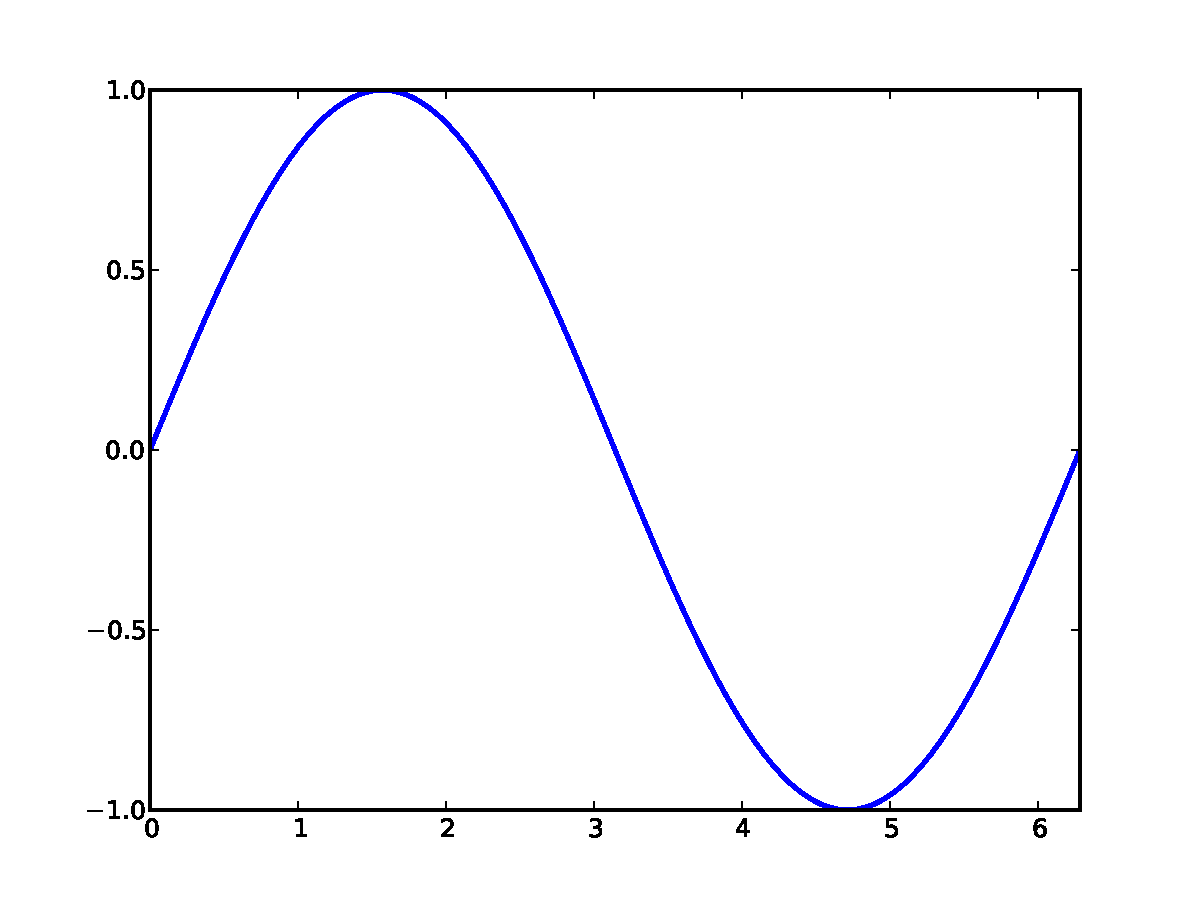
\includegraphics[width=. %
%   \textwidth]{sine}
%   \caption[Short caption for Table of Figures]{Illustration of how to
%   include a figure (long text, should not go to Table of Figures).} %
%   }
%   \label{fig:sine}
% \end{figure}





%%%%%%%%%%%%%%%%%%%%%%%%%%%%%%%%%%%%%%%%%%%%%%%%%%
% Keep the following \cleardoublepage at the end of this file,
% otherwise \includeonly includes empty pages. %
\cleardoublepage

% vim: tw=70 nocindent expandtab foldmethod=marker foldmarker={{{}{,}{}}}. %
